\documentclass[reprint,english,notitlepage]{revtex4-2}
\usepackage{amsmath}
\usepackage[mathletters]{ucs}
\usepackage[utf8x]{inputenc}
\usepackage[english]{babel}
\usepackage{esint}
\usepackage{physics,amssymb}
\usepackage{graphicx}
\usepackage{xcolor}
\usepackage{hyperref}
\usepackage{listings}
\usepackage{subfigure} 
\hypersetup{
    colorlinks,
    linkcolor={red!50!black},
    citecolor={blue!50!black},
    urlcolor={blue!80!black}}

\lstset{inputpath=,
	backgroundcolor=\color{white!88!black},
	basicstyle={\ttfamily\scriptsize},
	commentstyle=\color{magenta},
	language=Python,
	morekeywords={True,False},
	tabsize=4,
	stringstyle=\color{green!55!black},
	frame=single,
	keywordstyle=\color{blue},
	showstringspaces=false,
	columns=fullflexible,
	keepspaces=true}


\begin{document}



\title{Onboard Orientation Software}
\author{Oskar Idland \& Jannik Eschler}
\date{\today}
\affiliation{Institute of Theoretical Astrophysics, University of Oslo}

\begin{abstract}
    This is an abstract \colorbox{red}{Complete this summary at the end of the paper}
\end{abstract}
\maketitle

\section{Theory} \label{sec:theory}
For theory, see section \textbf{Relevant Mathematics} \colorbox{red}{Jannik legger in kilde} 
  


\section{Introduction} \label{sec:introduction}
As there is no up or down in space we will have to create our own way of navigating the cosmos. For this purpose we have made software capable of orientation in space. It will be able to calculate the angular orientation, find the velocity and get the position of the spacecraft. 


\section{Method} \label{sec:method}
A satellite is orbiting our home planet and has taken a $ 360 ^{o} × 360 ^{o} $ picture of the entire sky where all positions are described using spherical coordinates. As the stars and galaxies as very far away we are going to assume the pictures looks the same from the perspective of our shuttle. Using this picture we can create a stereographic projection as a means to convert from spherical coordinates to planar coordinates. Comparing the picture taken from a camera at on the shuttle we can find our orientation.   
\begin{figure}[h!]
  \centering
  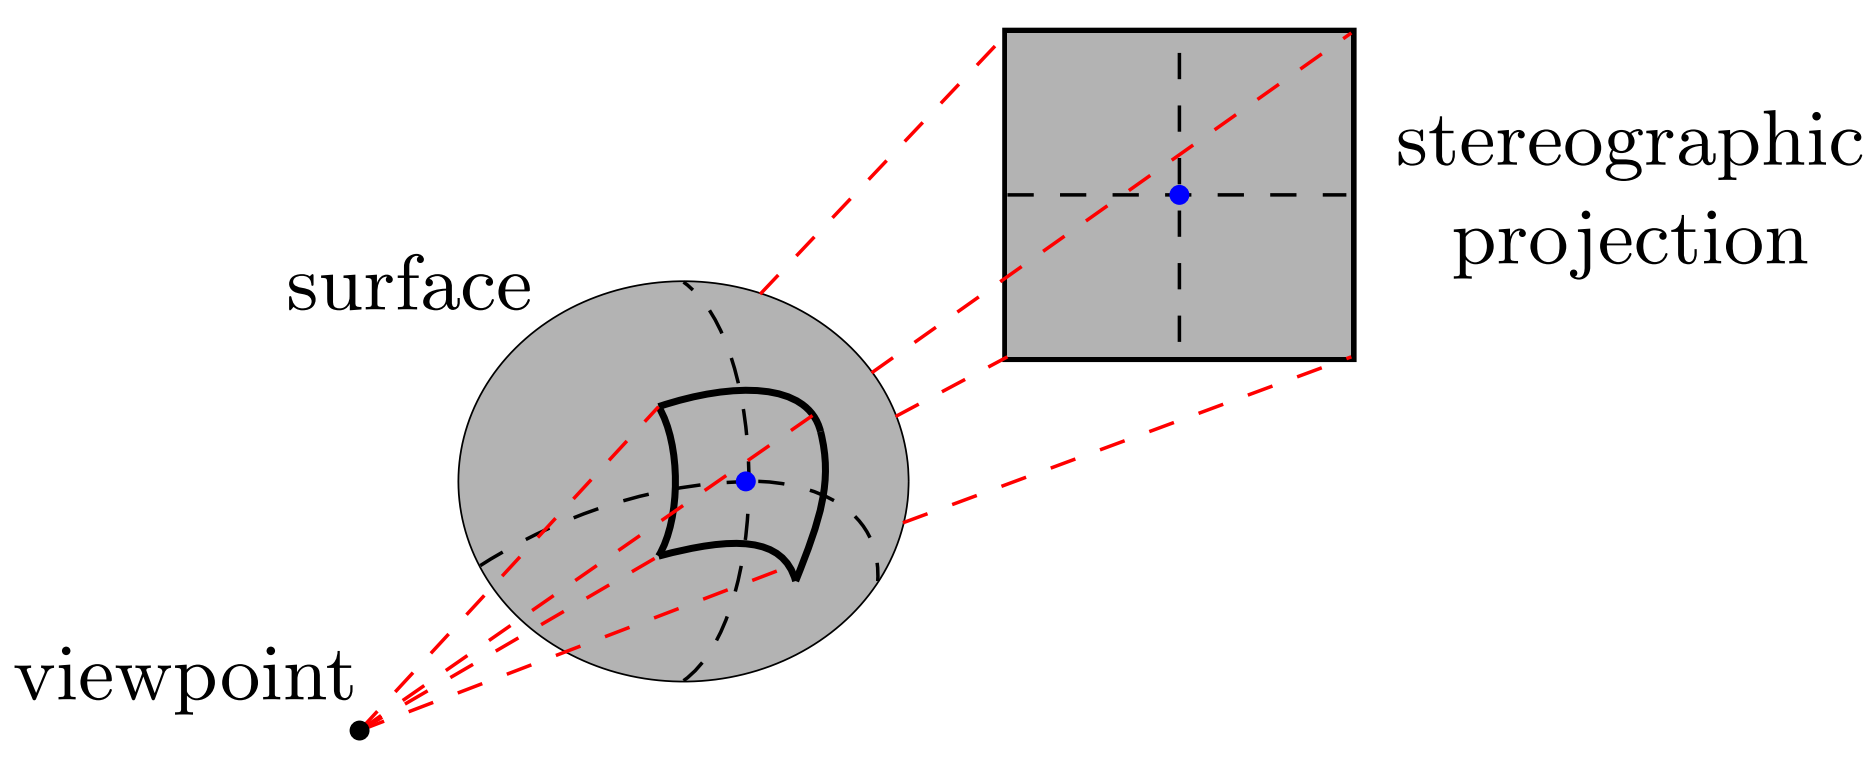
\includegraphics[scale = .2]{Figures/Stereographic_projection.png}
  \caption{Illustration of stereographic projection}
  \label{fig: Stereographic Projection}
\end{figure}
To relate the spherical coordinates $ \theta, \phi $ to the planar coordinates $ X, Y $ we use the following equations \colorbox{red}{Husk å ta med utledning} :
\begin{equation} \label{Spherical to X}
	X = κ  \sin θ \sin (ϕ - ϕ _0)
\end{equation}
\begin{equation}\label{Spherical to Y}
	Y = κ (\sin θ _0 \cos  θ - \cos θ _0 \sin θ \cos (ϕ - ϕ _0))  
\end{equation}



\section{Results} \label{sec:results}



\section{Discussion} \label{sec:discussion}



\section{Conclusion} \label{sec:conclusion}






\section{Appendix: Mathematical Derivations}

\newpage 

\end{document}